\documentclass[11pt]{article}
\usepackage{graphicx}
\usepackage{float}
\usepackage{amsmath}
\usepackage{amsfonts}
\usepackage[brazilian]{babel}
\usepackage[utf8]{inputenc}
\usepackage[T1]{fontenc}

\begin{document}

\title{Tipos de funções - Funções exponenciais}
\author{Erik Perillo}
\date{}
\maketitle
\begin{abstract}
Vamos agora falar de funções exponenciais.
\end{abstract}

\newpage

\tableofcontents

\newpage

\section{A cara de uma função exponencial}
\par
Uma função exponencial é uma da forma:
$$f(x) = a^x$$
Ou seja, é $a$ \emph{elevado} a $x$. Pode haver dois casos:
\begin{itemize}
	\item $a > 1$
	\item $a < 1$
\end{itemize}

\paragraph{}
Quando $a > 1$, a função é crescente. Pegue o exemplo $f(x) = 2^x$. Quando 
$x = 0$, $f(x) = 0$. Quando $x = 1$, $f(x) = 2$ e assim por diante. 
Se desenharmos a função, teremos algo como:
\begin{figure}[H]
	\centering
	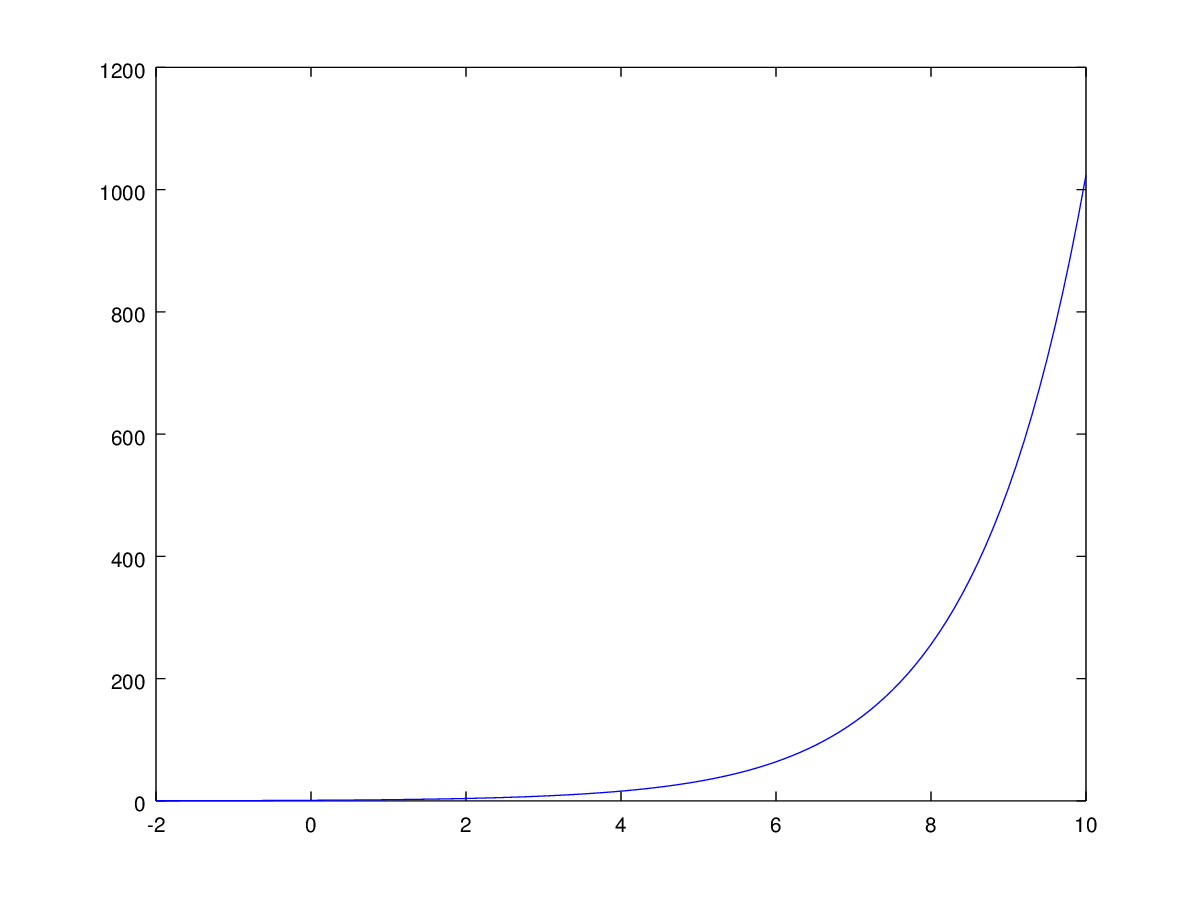
\includegraphics[width=0.7\linewidth]{imgs/exp.png}
\end{figure}
Veja que, para $x < 0$, ela \emph{tende} a zero, mas \textbf{nunca} é zero.
Para $x > 0$, ela cresce \emph{muito} rápido.
\paragraph{}
Quando $a < 1$, a função é decrescente. Imagine que é porque você está pegando
um número (a) que é menor que 1 e multiplicando-o por ele mesmo. Por exemplo,
$0.5$: 
$$0.5*0.5 = 0.5^2 = 0.25$$ 
O que é menor que $0.5$. Quanto mais você
multiplica o número por ele mesmo, menor ele fica.
\par
Pegue como exemplo $f(x) = {(\frac{1}{2})}^x$. A função fica com esta cara:
\begin{figure}[H]
	\centering
	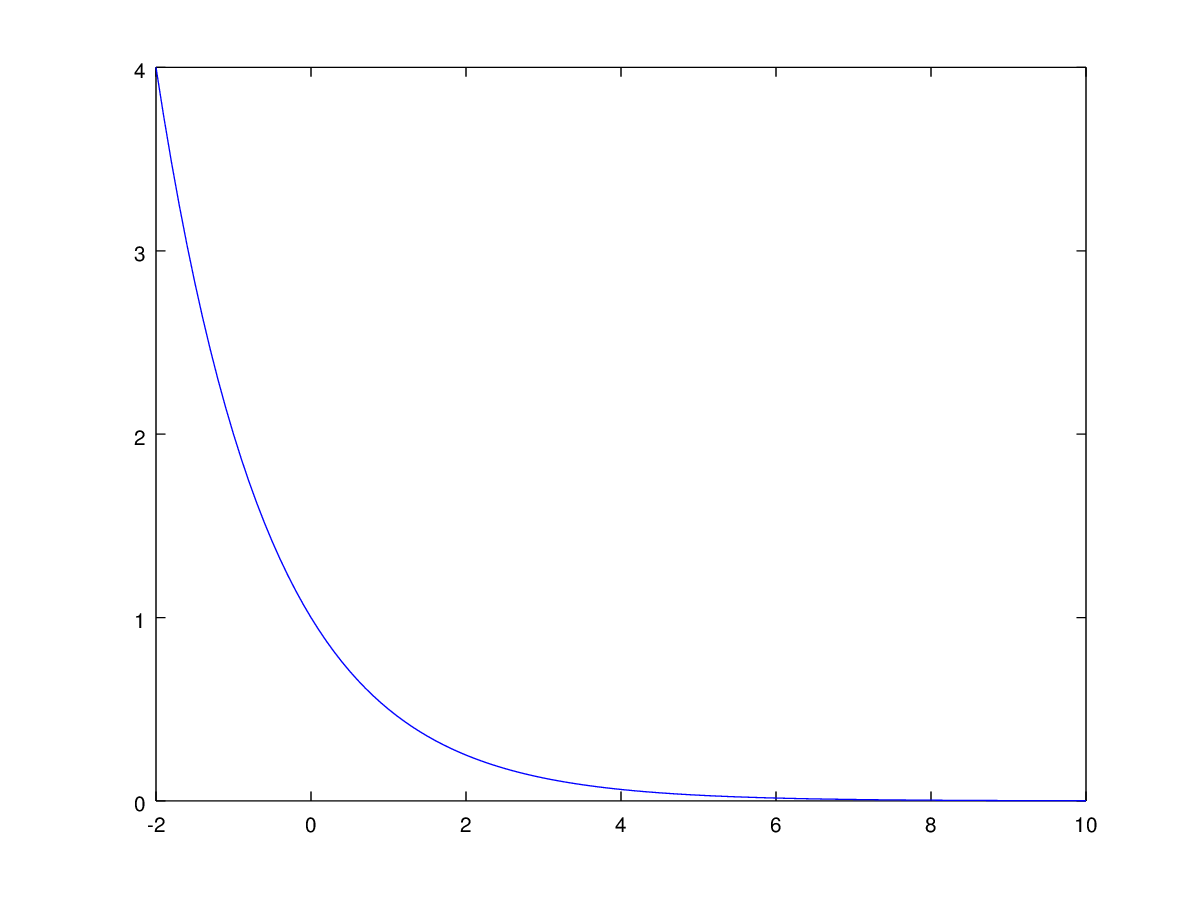
\includegraphics[width=0.7\linewidth]{imgs/exp_inv.png}
\end{figure}
\paragraph{}
Note que, se tivéssemos algo como $f(x) = 2^{-x}$, a função seria decrescente.
Isso porque conseguimos reescrever isso como $f(x) = {(2^{-1})}^x = 
{(\frac{1}{2})}^x$ e, nesse caso, a vira menor que 1. 
A mesma coisa pra se $a < 1$ e x for negativo: ela vira crescente ao invés de
decrescente.
\paragraph{}
Qualquer que seja a função exponencial, ela \emph{sempre vai ser 1 com $x=0$},
ou seja, sempre vai cruzar o eixo y em $y=1$. Isso porque qualquer número
elevado a $0$ é $1$.

\newpage{}

\section{Exercícios}
\begin{enumerate}
	\item Diga se as funções a seguir são crescentes ou decrescentes.
	\begin{enumerate}
		\item $f(x) = 3^x$
		\item $f(x) = 2^{-x}$
		\item $f(x) = {0.28}^{2x}$
		\item $f(x) = {\left(\frac{1}{4}\right)}^{-x}$
		\item $f(x) = -2^x$
	\end{enumerate}

	\item Esboce o gráfico das funções a seguir.
	\begin{enumerate}
		\item $f(x) = {1.618}^x$
		\item $f(x) = 1^x$
		\item $f(x) = {0.618}^x$
	\end{enumerate}
\end{enumerate}

\newpage{}

\section{Respostas aos Exercícios}

\begin{enumerate}
	\item
	\begin{enumerate}
		\item Crescente.
		\item Decrescente.
		\item Decrescente.
		\item Crescente.
		\item Descrescente.
	\end{enumerate}

	\item Esboce o gráfico das funções a seguir.
	\begin{enumerate}
		\item --
			\begin{figure}[H]
				\centering
				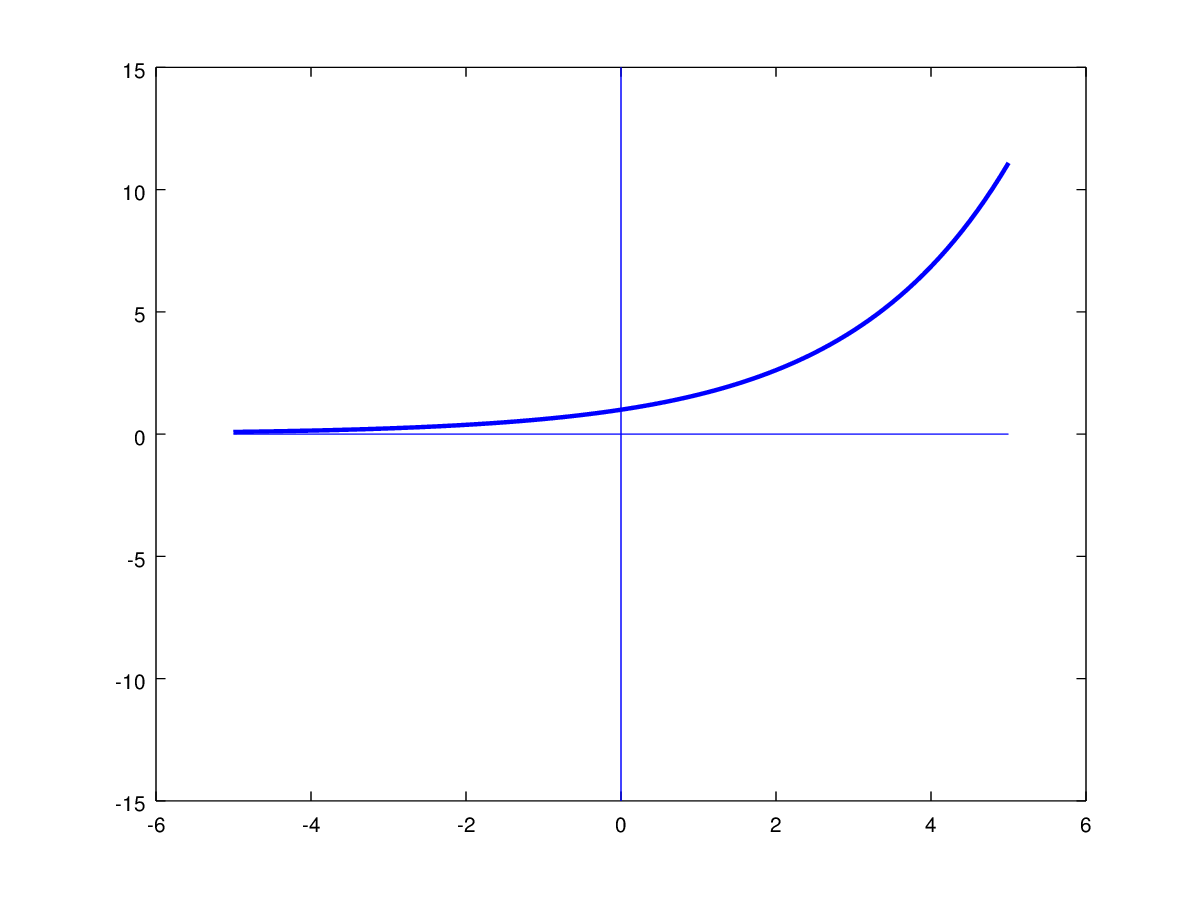
\includegraphics[width=0.7\linewidth]{imgs/ex2a.png}
			\end{figure}
		\item --
			\begin{figure}[H]
				\centering
				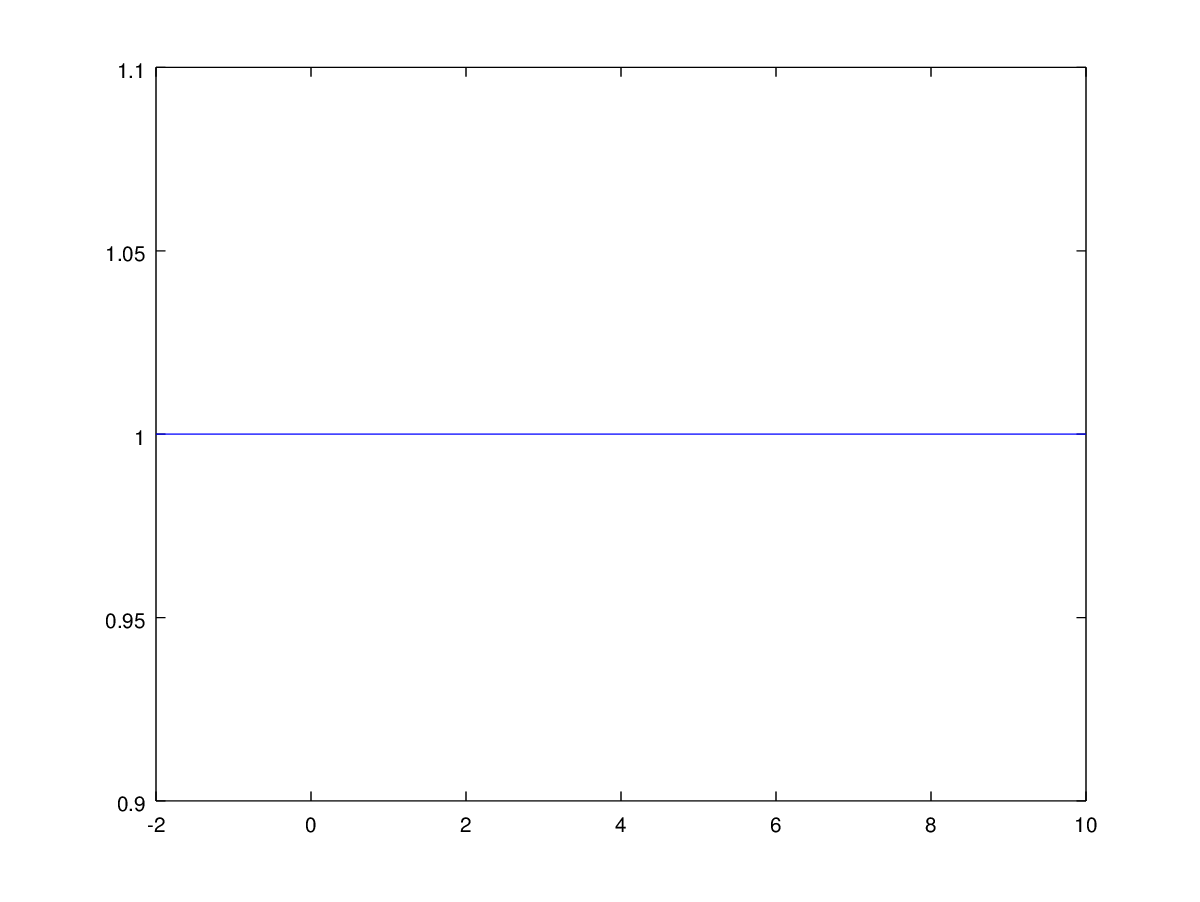
\includegraphics[width=0.7\linewidth]{imgs/ex2b.png}
			\end{figure}
		\item --
			\begin{figure}[H]
				\centering
				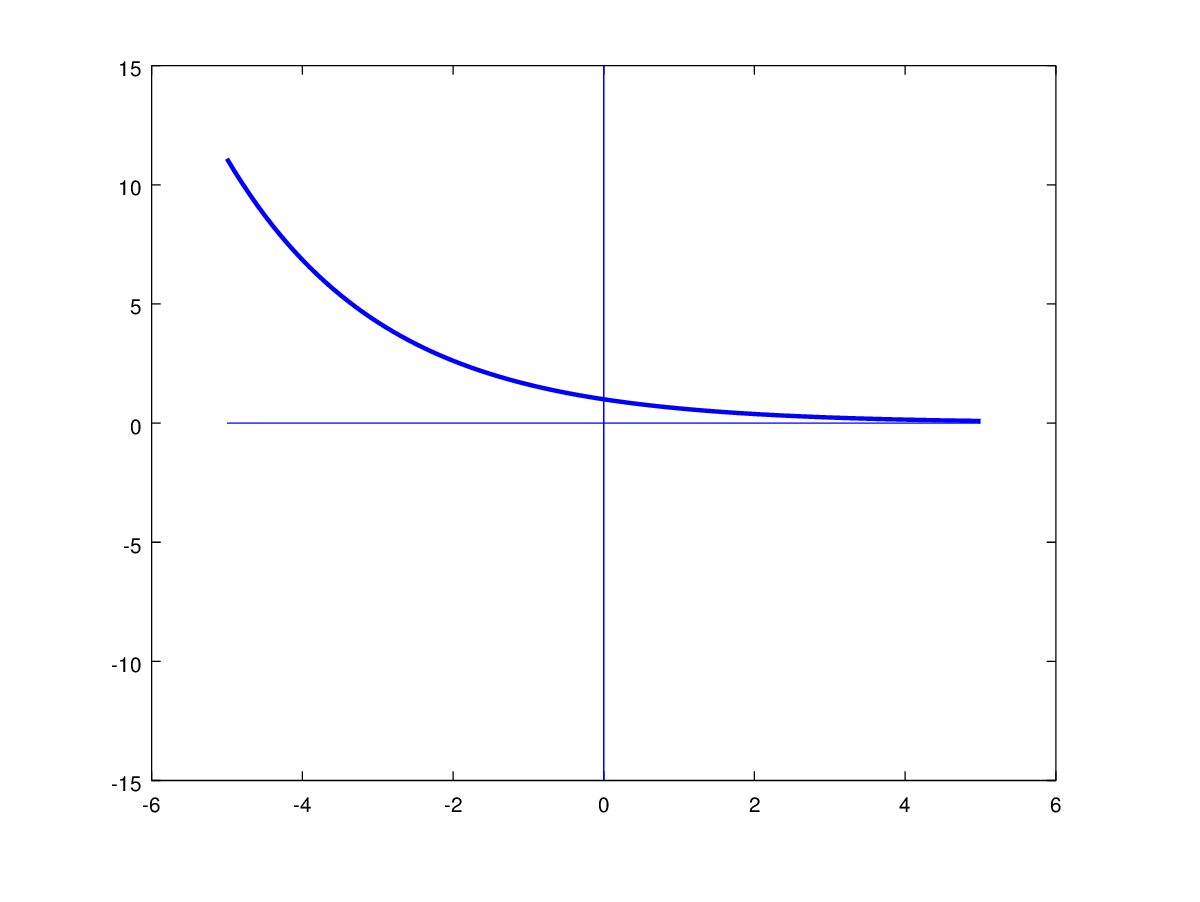
\includegraphics[width=0.7\linewidth]{imgs/ex2c.png}
			\end{figure}
	\end{enumerate}
\end{enumerate}

\end{document}
